\section{Introduction} \label{sec:intro}
% What leads to distribution of heavy elements in a galaxy
Many elements heavier than hydrogen are produced through nuclear fusion in compact objects such as supernovae, dying low mass stars, and neutron star-neutron star mergers \citep[e.g.][]{2023A&ARv..31....1A}. By necessity, stars inherit the constituitive properties of the gas from which they formed. Moreover, the surface abundance of most elements for most stars do not change over most of their lifetime. We therefore have the opportunity to examine the historical record of the gas-phase abundance of a galaxy by way of the distribution of the surface abundances of stars.

The enrichment of the gas-phase of a galaxy is determined by a complicated combination of physical processes - stellar evolution and supernovae, gas accretion, mergers, gas outflows from stellar and AGN feedback, metal mixing and diffusion, etc. Because the processes which give rise to this distribution are complex, there is almost certainly some structure in the stellar abundance distribution for every galaxy. However, it has only been definitively measured in the Milky Way (there is a claim of no measured structure in M31 by \citet{2024IAUS..377..115N}).

% How present-day stellar surface abundances are linked to history of gas-phase abundances

% Why alpha-elements are important
The distribution of elemental abundances is a high dimensional space \citep[e.g., 32 elements in][]{2024ApJ...961L..41J}. However, this space is highly degenerate, and so the effective number of dimensions is much smaller -- even possibly compressed to just \FeH{} and age \citep{2019ApJ...883..177N}. Two elements have received particular interest - Fe and elements produced by the $\alpha$-process. Type Ia and Type II supernovae are the main contributors of Fe and $\alpha$ enrichment. Fe is broadly produced in both types, and so its abundance is a proxy for the total metallicity of a star. On the other hand, $\alpha$-elements are mainly produced in Type II supernovae. The ratio of $\alpha$-elements to Fe (\alphaFe{}) is then a measure of the relative contributions of Type Ia and II SNe to the enrichment of a parcel of gas. It has therefore become common to compress the high-dimensional abundance space to the two dimensional \alphaFe{}-\FeH{} plane.

% Observed chemical bimodality in the Milky Way
It is now well-established that, in the Milky Way, a bimodality exists in the \alphaFe{}-\FeH{} plane \citep{1996ASPC...92..307G,1998A&A...338..161F,2004AN....325....3F,2006MNRAS.367.1329R,2011A&A...535L..11A,2012A&A...545A..32A,2014A&A...562A..71B,2014ApJ...796...38N,2020MNRAS.493.2952H}. This bimodality is typically separated into the high-$\alpha$ and low-$\alpha$ sequences. These sequences are also associated with differences in their physical extent -- the high-$\alpha$ sequence is more centrally compact and vertically extended than the low-$\alpha$ sequence.

% Different explanations of bimodality
Naturally, many different processes that could lead to structure in the abundance plane have been discussed in the literature. An early explanation of the bimodality is the two-phase gas infall model \citep{1997ApJ...477..765C,2009IAUS..254..191C,2017MNRAS.472.3637G,2019A&A...623A..60S}. In this model, the thick disk first forms rapidly from an initial infall of gas. Because the typical SFR is high, these stars are $\alpha$-enhanced. In some variants, star formation halts completely before a second supply of pristine gas falls into the Galaxy \citep[][and references therein]{2024arXiv240511025S}. This dilutes the gas supply from which the thin disk forms more gradually. The thin disk is then more $\alpha$-poor because its associated SFR is lower.

A later argument by \citet{2021MNRAS.501.5176K} asserts that the two sequences follow from two phases of gas infall, except driven by stellar feedback instead of cosmological inflow. An initial bursty phase follows from the direct collapse of the gaseous halo. The disk has a high SFR leading to the formation of the high-$\alpha$ sequence. Feedback then halts the inflow, and a slower accretion of high-angular momentum and metal-rich gas commences, forming the low-$\alpha$ sequence.

Another mechanism to generate structure in the abundance plane was pointed out by \citet{2009MNRAS.396..203S}, further developed by \citet{2021MNRAS.507.5882S,2023MNRAS.523.3791C}, and explored by \citet{2011ApJ...737....8L,2021MNRAS.508.4484J}. This model claims that, since stars are thought to migrate from their birth radius, there will be stars throughout the entire disk that formed in the inner disk. These $\alpha$-enhanced stars will then form the high-$\alpha$ sequence. This model and its variants also match some chemodynamic properties of the disk. One salient feature of these models is that the bimodality can result from a smooth star formation history.

Yet another explanation, which also invokes an internal process, is that the formation of clumps at high redshift are responsible for both the chemistry and dynamics of the high-$\alpha$ sequence \citep{2019MNRAS.484.3476C,2020MNRAS.492.4716B,2021MNRAS.502..260B,2023ApJ...953..128G}. Instabilities are thought to form clumps in gas-rich disks, and such clumps are seen at intermediate redshifts \citep[$z\sim2$;][]{2005ApJ...627..632E,2007ApJ...658..763E}. These clumps then self-enrich, forming $\alpha$-enhanced stars. The high-$\alpha$ sequence stops forming once the gas fraction is low enough for the instabilities to no longer arise. This model predicts that the high-$\alpha$ and low-$\alpha$ sequences form simultaneously.

Next, we turn to models which argue the bimodality results from some external influence. Early arguments were made that both the $\alpha$-enhancement of the disk and the thickening of the disk can result from gas-rich mergers \citep{2004ApJ...612..894B,2005ApJ...630..298B,2007ApJ...658...60B,2010MNRAS.402.1489R}.\footnote{See also \citet{2009MNRAS.400.1347C} for an argument invoking semi-analytic models.} These mergers lead to an enhanced SFR which leads to the $\alpha$-enhancement of the thick disk.

In cosmological simulations, which naturally include early gas-rich mergers, the situation is not as clear. Early work by \citet{2012MNRAS.426..690B} found a general separation between the thin and thick disk, though other authors found a smooth evolution \citep{2013A&A...558A...9M}. \citet{2018MNRAS.474.3629G} found what they referred to as a chemical dichotomy, and argued that it can come from either gas-rich mergers as described before or a ``compaction'' of the disk (we will return to this point in Section~\ref{ssec:cosmo}). Other authors highlight the metal content of the infalling gas, stating that the metal-poor gas associated with satellites can suddenly dilute or reset the disk's metallicity \citep{2020MNRAS.491.5435B,2024MNRAS.528L.122C}. This interpretation can also be understood in the framework of the two-infall models.

The merger explanation of the bimodality is highly synergistic with our picture of the hierarchical assembly of the stellar halo \citep{2005ApJ...635..931B}. Indeed, there is strong evidence that the Milky Way underwent a significant merger with the so-called Gaia-Sausage-Enceladus satellite \citep[GSE;][]{2018MNRAS.478..611B,2018Natur.563...85H,2020ApJ...901...48N}. This merger is thought to have occurred $\sim8-10\,\Gyr$ ago \citep[see also][]{2020ApJ...897L..18B}.

Claims in the literature on the stellar mass of GSE vary widely. Early estimates argued from $6\times10^8$ up to even $10^{10}\,\Msun$ \citep{2018MNRAS.478..611B,2018Natur.563...85H,2019MNRAS.484.4471F,2019MNRAS.487L..47V,2019MNRAS.488.1235M,2020MNRAS.493.5195D,2020MNRAS.497..109F}. Later estimates have been more conservatives with estimates from a mass of $3\times10^8\,\Msun$ to $10^9\,\Msun$ \citep{2019MNRAS.482.3426M,2020MNRAS.492.3631M,2021ApJ...923...92N,2022AJ....164..249H}, and even as low as $1.5\times10^8\,\Msun$ \citep{2023MNRAS.526.1209L}.

In this work, we explored an idealized simulation which resembles the merger between the Milky Way and GSE. We found that in certain configurations, which have only minor differences in their orbit, a bimodal distribution of stellar abundances in the \alphaFe{}-\FeH{} plane is produced. This is shown in Figure~\ref{fig:fig1}. The configurations which produce a bimodality are associated with a starburst followed by a quiescent phase followed by rejuvenation $\sim300\,\Myr$ later.

In Section~\ref{sec:methods}, we describe our setup. In Section~\ref{sec:results}, we present the main results of our simulations. In Section~\ref{sec:discussion}, we discuss and interpret our results, as well as connections to previous and future work, before concluding in Section~\ref{sec:conclusion}. Throughout this work we refer to the standard native time unit $\kpc/\left(\kms\right)$ as \Gyr{} for convenience.

\begin{figure*}
  \centering
  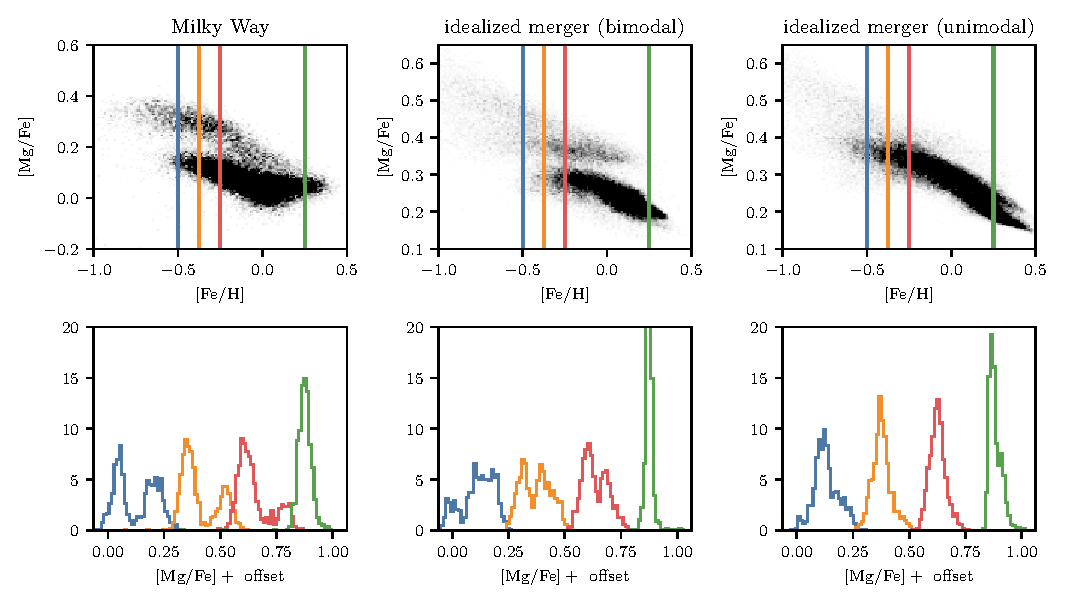
\includegraphics[width=\textwidth]{figure1.pdf}
  \caption{\textbf{The abundance bimodality seen in the Milky Way can be reproduced in some idealized merger simulations.} In the upper panels, we show the distribution of stars in the \MgFe{}-\FeH{} plane. The lower panels show the distribution of \MgFe{} at a fixed \FeH{} bin of width $0.05\,\dex$. The colors indicate the fixed \FeH values, which are $-0.5$, $-0.25$, $0$, and $0.25$. The left column shows the observed distribution in the Milky Way from ASPCAP DR17 \citep[][J.A.~Holtzman et al., in preparation]{2016AJ....151..144G}, while the right two columns show two idealized merger simulations. The idealized merger simulations are nearly identical, except that in the bimodal simulation the satellite has a starting radius of $129\,\kpc$, while in the unimodal simulation it has a starting radius of $142\,\kpc$. The labels ``unimodal'' and ``bimodal'' are of the \textit{outcome} of the simulation, and do not reflect a particular choice in the setup. The Milky Way (left column) exhibits a strong bimodal distribution of \MgFe{} at various \FeH{}. The idealized merger simulation marked as bimodal (center column) also exhibits a bimodal distribution of \MgFe{}, though the structure is not as strongly defined. The idealized merger simulation marked as unimodal (right column) exhibits only weak structure, if any at all.}
  \label{fig:fig1}
\end{figure*}